\documentclass[11pt,a4paper]{article}

\usepackage[a4paper,margin=1in]{geometry}
\usepackage[T1]{fontenc}
\usepackage{lmodern}
\usepackage{booktabs}
\usepackage{amsmath}
\usepackage{pgfplots}
\usepackage{xcolor}

\pgfplotsset{compat=1.17}
\setlength{\parindent}{0pt}
\setlength{\parskip}{6pt}
\renewcommand{\arraystretch}{1.15}

\begin{document}

\begin{center}
{\Large Selected Numerical Results for the Hybrid LSMC--PDE Method}\\[0.5em]
{\normalsize BGK-style calibrated gDMR model with 12 Bermudan exercise dates}\\[0.5em]
{\normalsize 27 March 2026}
\end{center}

\section*{1. Experimental Setting}

The experiments in this note use the BGK-style calibrated gDMR specification
\[
S_0 = 100,\quad v_0 = 0.114,\quad v'_0 = 0.110,\quad r = 0,\quad T = 1,
\]
with
\[
\kappa_1 = 5.5,\quad \kappa_2 = 0.1,\quad \theta = 0.078,\quad \xi_1 = 2.689,\quad \xi_2 = 0.502,
\]
and
\[
\delta_1 = \delta_2 = 0.94,\quad \rho_{12} = -0.982,\quad \rho_{13} = -0.727,\quad \rho_{23} = 0.59.
\]
The Bermudan contract is sampled at \(12\) exercise dates. Three strike levels are considered:
\[
K \in \{90, 100, 110\},
\]
corresponding to OTM, ATM, and ITM puts.

The benchmark method is standard LSMC. The hybrid method couples LSMC with a PDE correction on a one-dimensional asset grid. In the tuned hybrid runs reported below, the common numerical setting is
\[
\text{paths} = 60{,}000,\quad \text{asset points} = 301,\quad
S_{\min}/S_0 = 0.30,\quad S_{\max}/S_0 = 3.50,
\]
with volatility truncation quantile \(0.999\).

For any direct price estimate \(\widehat{V}\) and reference value \(V^{\mathrm{ref}}\), the direct relative error is defined by
\[
\varepsilon_{\mathrm{dir}} = \frac{\lvert \widehat{V} - V^{\mathrm{ref}} \rvert}{\lvert V^{\mathrm{ref}} \rvert}.
\]

\section*{2. Tuned Comparison Across Moneyness}

The first experiment fixes \(12\) exercise dates and compares the tuned hybrid method with the benchmark LSMC under the original BGK-style production setting with \(600\) Euler steps. The benchmark uses \(10^6\) paths, while the tuned hybrid uses \(60{,}000\) paths.

\begin{table}[h!]
\centering
\caption{Direct-price comparison under the tuned hybrid setting.}
\begin{tabular}{lcccc}
\toprule
Scenario & \(K\) & Benchmark direct & Hybrid direct & Hybrid dir. err. \\
\midrule
ATM & 100 & 11.371204 & 11.359836 & 0.100\% \\
ITM put & 110 & 16.637388 & 16.680641 & 0.260\% \\
OTM put & 90 & 7.426156 & 7.414778 & 0.153\% \\
\bottomrule
\end{tabular}
\end{table}

The tuned hybrid method achieves direct relative errors below \(0.3\%\) in all three moneyness regimes. In particular, the ATM and OTM cases are reduced to \(0.100\%\) and \(0.153\%\), respectively, while the ITM case remains at \(0.260\%\).

\section*{3. Path-Count Study at 48 Euler Steps}

To study the direct estimator under a coarser time discretization, a path-count sweep was run with Euler steps fixed at \(48\). For this comparison, the reference prices were strengthened by using benchmark-only runs with \(1200\) Euler steps and \(1{,}200{,}000\) benchmark paths:
\[
V^{\mathrm{ref}}_{\mathrm{ATM}} = 11.356823,\qquad V^{\mathrm{ref}}_{\mathrm{OTM}} = 7.402999.
\]

The results are especially favorable to the hybrid method. For both ATM and OTM, the hybrid direct error remains below the LSMC benchmark error at every tested path count from \(250\) to \(60{,}000\).

\begin{table}[h!]
\centering
\caption{Representative direct relative errors at 48 Euler steps, rebased to the 1200-step benchmark reference.}
\begin{tabular}{llcc}
\toprule
Scenario & Paths & Benchmark dir. err. & Hybrid dir. err. \\
\midrule
ATM & 1,000 & 6.053\% & 1.620\% \\
ATM & 10,000 & 1.806\% & 0.960\% \\
ATM & 20,000 & 1.336\% & 0.052\% \\
ATM & 60,000 & 1.232\% & 0.302\% \\
\midrule
OTM put & 1,000 & 7.840\% & 2.905\% \\
OTM put & 10,000 & 2.877\% & 0.869\% \\
OTM put & 20,000 & 2.173\% & 0.248\% \\
OTM put & 60,000 & 1.769\% & 0.526\% \\
\bottomrule
\end{tabular}
\end{table}

\begin{figure}[p]
\centering
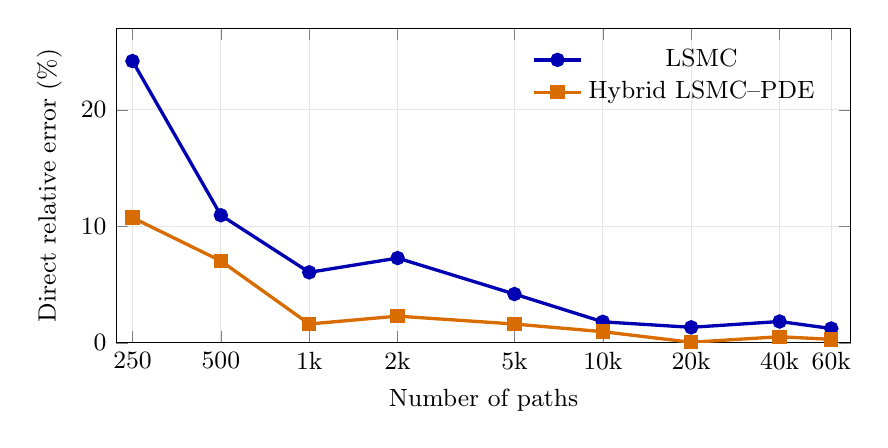
\begin{tikzpicture}
\begin{axis}[
    width=0.9\textwidth,
    height=0.46\textwidth,
    xmode=log,
    log basis x={10},
    xmin=220,
    xmax=70000,
    ymin=0,
    ymax=27,
    xlabel={Number of paths},
    ylabel={Direct relative error (\%)},
    xtick={250,500,1000,2000,5000,10000,20000,40000,60000},
    xticklabels={250,500,1k,2k,5k,10k,20k,40k,60k},
    ymajorgrids=true,
    xmajorgrids=true,
    grid style={draw=gray!20},
    tick label style={font=\small},
    label style={font=\small},
    legend style={draw=none, fill=none, font=\small, at={(0.97,0.97)}, anchor=north east},
    every axis plot/.append style={very thick},
]
\addplot[color=blue!70!black, mark=*] coordinates {
    (250,24.184)
    (500,10.954)
    (1000,6.053)
    (2000,7.278)
    (5000,4.190)
    (10000,1.806)
    (20000,1.336)
    (40000,1.834)
    (60000,1.232)
};
\addlegendentry{LSMC}
\addplot[color=orange!85!black, mark=square*] coordinates {
    (250,10.745)
    (500,7.032)
    (1000,1.620)
    (2000,2.295)
    (5000,1.618)
    (10000,0.960)
    (20000,0.052)
    (40000,0.529)
    (60000,0.302)
};
\addlegendentry{Hybrid LSMC--PDE}
\end{axis}
\end{tikzpicture}
\caption{ATM direct relative error at 48 Euler steps, rebased to the 1200-step benchmark reference.}
\end{figure}

\begin{figure}[p]
\centering
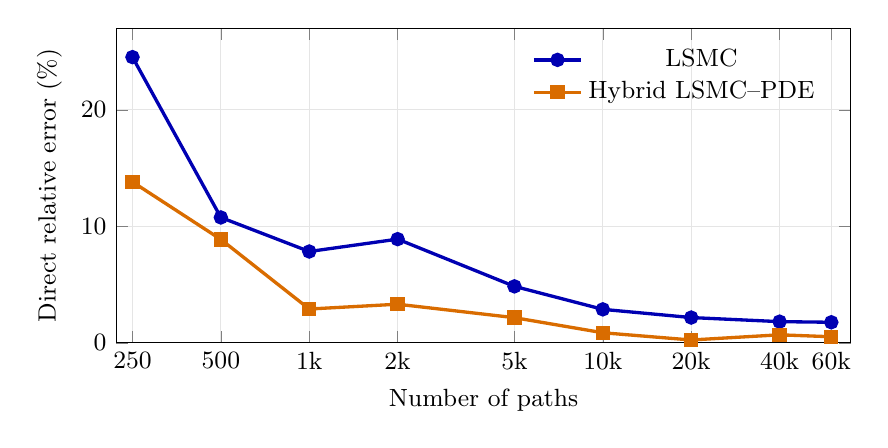
\begin{tikzpicture}
\begin{axis}[
    width=0.9\textwidth,
    height=0.46\textwidth,
    xmode=log,
    log basis x={10},
    xmin=220,
    xmax=70000,
    ymin=0,
    ymax=27,
    xlabel={Number of paths},
    ylabel={Direct relative error (\%)},
    xtick={250,500,1000,2000,5000,10000,20000,40000,60000},
    xticklabels={250,500,1k,2k,5k,10k,20k,40k,60k},
    ymajorgrids=true,
    xmajorgrids=true,
    grid style={draw=gray!20},
    tick label style={font=\small},
    label style={font=\small},
    legend style={draw=none, fill=none, font=\small, at={(0.97,0.97)}, anchor=north east},
    every axis plot/.append style={very thick},
]
\addplot[color=blue!70!black, mark=*] coordinates {
    (250,24.521)
    (500,10.762)
    (1000,7.840)
    (2000,8.902)
    (5000,4.849)
    (10000,2.877)
    (20000,2.173)
    (40000,1.823)
    (60000,1.769)
};
\addlegendentry{LSMC}
\addplot[color=orange!85!black, mark=square*] coordinates {
    (250,13.812)
    (500,8.877)
    (1000,2.905)
    (2000,3.318)
    (5000,2.163)
    (10000,0.869)
    (20000,0.248)
    (40000,0.693)
    (60000,0.526)
};
\addlegendentry{Hybrid LSMC--PDE}
\end{axis}
\end{tikzpicture}
\caption{OTM direct relative error at 48 Euler steps, rebased to the 1200-step benchmark reference.}
\end{figure}

\clearpage
\section*{4. Additional Check at 60 Euler Steps}

An additional saved comparison is available at \(60\) Euler steps. Rebased to the same \(1200\)-step benchmark references, the hybrid method still produces smaller direct errors for both ATM and OTM:

\begin{table}[h!]
\centering
\caption{Direct relative error at 60 Euler steps under the stronger benchmark reference.}
\begin{tabular}{lcccc}
\toprule
Scenario & Benchmark direct & Hybrid direct & Benchmark dir. err. & Hybrid dir. err. \\
\midrule
ATM & 11.381616 & 11.350391 & 0.218\% & 0.057\% \\
OTM put & 7.435732 & 7.410080 & 0.442\% & 0.096\% \\
\bottomrule
\end{tabular}
\end{table}

Although the hybrid advantage is strongest at \(48\) Euler steps, the saved \(60\)-step check indicates that the improvement in direct pricing accuracy persists when the time grid is moderately refined.

\section*{5. Conclusion}

The experiments reported here support the following conclusions.

\begin{itemize}
\item With \(12\) exercise dates and the tuned numerical setting, the hybrid method delivers accurate prices across ATM, ITM, and OTM cases, with direct relative errors below \(0.3\%\).
\item At a coarse Euler grid of \(48\) steps, the hybrid direct estimator is uniformly more accurate than the benchmark LSMC estimator over the full tested path range in both ATM and OTM cases, even when the reference is strengthened to a \(1200\)-step, \(1.2\) million-path benchmark.
\item The saved \(60\)-step comparison remains favorable to the hybrid method, suggesting that the improvement is not confined to the most extreme coarse-grid regime.
\end{itemize}

Taken together, these results indicate that the hybrid LSMC--PDE method is particularly effective when high-quality direct prices are required under a relatively coarse time discretization, while still maintaining good accuracy across different moneyness regimes.

\end{document}
